\documentclass{article} 
\usepackage[utf8]{inputenc}
\usepackage{ amssymb, systeme,   float, graphicx, fontawesome5, titlesec, tabularray, esvect}
\usepackage[most]{tcolorbox}
\usepackage[scale=.95,type1]{cabin}
\usepackage[framemethod=tikz]{mdframed}


\usepackage[legalpaper,margin=1in]{geometry}

\setlength{\parindent}{10pt}
\setlength{\parskip}{1em}
\renewcommand{\baselinestretch}{1.2}

\title{3 }
\date{}
\author{}

\newcounter{Def}[section]
\newenvironment{Def}[1][]{
  \ifstrempty{#1}%
  {\mdfsetup{%
    frametitle={%
      \tikz[baseline= (current bounding box.east),outer sep=0pt]
      \node[line width=1pt,anchor=east,rectangle,draw=blue!20,fill=white]
      {\strut \color{black}{Definition}~};}}
  }%
  {\mdfsetup{%
    frametitle={%
      \tikz[baseline= (current bounding box.east),outer sep=0pt]
      \node[line width=1pt,anchor=east,rectangle,draw=blue!20,fill=white]
    {\strut \color{black}{Definition}~:~\color{blue4}{#1}};}}%
  }%
  \mdfsetup{innertopmargin=2pt,linecolor=blue!20,%
            linewidth=1pt,topline=true,%
            frametitleaboveskip=\dimexpr-\ht\strutbox\relax,}
  \begin{mdframed}[]\relax%
}{\end{mdframed}}

\titleformat{\section}
  {\fontfamily{lmss}\selectfont\LARGE\bfseries\color{black}}
  {\thesection}{1em}{}  
\begin{document}
\section{Directional Derivatives and the Gradient Vector}

\begin{minipage}[]{0.5\linewidth}
  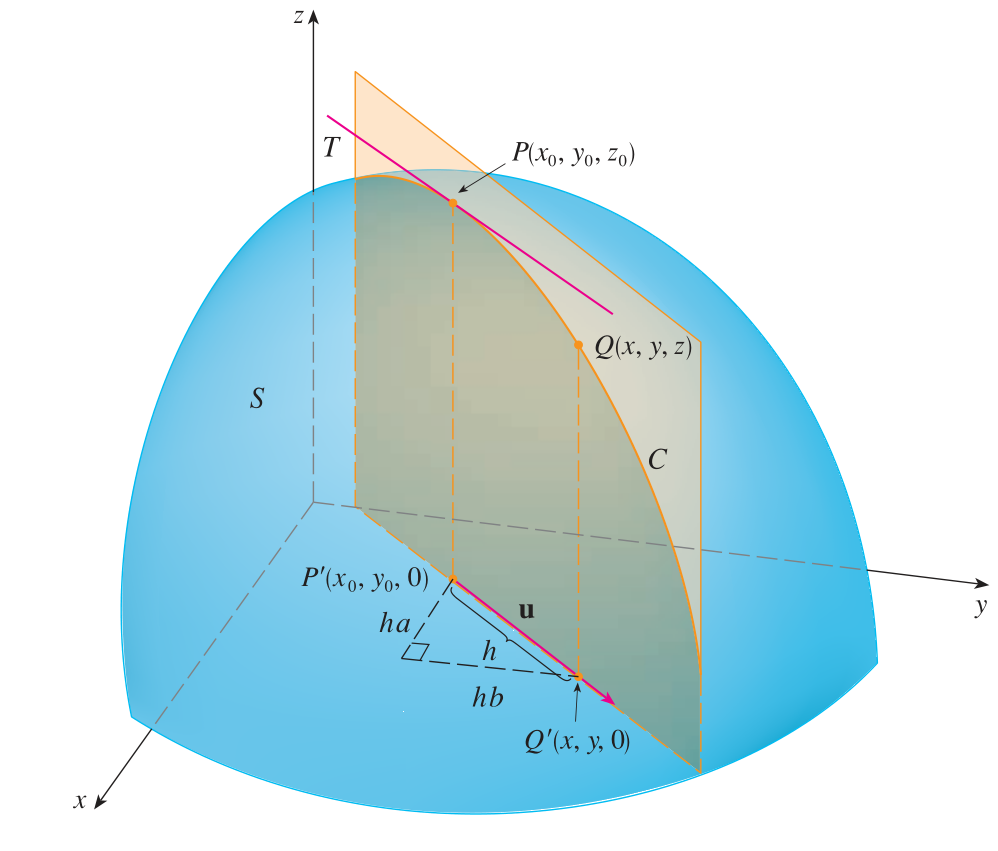
\includegraphics[width = 8 cm]{./images/grad.png}
  
\end{minipage}
\begin{minipage}[]{0.47\linewidth}
\subsection*{{\fontfamily{lmss}\selectfont \textcolor{blue5}{\faIcon{anchor} \underline{Directional Derivatives}}}}
We want the rate of change of $z$ at $(x _ 0, y _ 0 )$ in the direction of an unit vector \textbf{u} = $\langle a, b  \rangle$. 

\textcolor{blue5}{\faIcon{caret-right}} Consider the surface $S$ of $z = f(x,y)$, the vertical plane that passes through $P(x_0, y_0, z_0)$  in the direction of \textbf{u} intersects $S$ a curve $C$. 

\textcolor{blue5}{\faIcon{caret-right}} The slope of tangent line $T$ to $C$ at $P$ is what we need.
\end{minipage}

If $Q(x,y,z)$ is another point on $C$ and $P', Q'$ are the projections of $P, Q$ onto the $xy$-plane, then the vector $\vv{P'Q'}$ is parallel to \textbf{u}, 
\[\vv{P'Q'} = h \textbf{u} = \langle ha, hb  \rangle  \]
Therefore $x - x_0 = ha$, $y - y_0 = hb $.
\[ \cfrac{\Delta z }{h } = \cfrac{z - z_0 }{h } = \cfrac{f(x_0 + ha, y_0 + hb ) - f(x_0, y_0)}{h}\]
If we take limit as $h \to 0 $, we obtain the rate of change of $z $ (with respect to distance) in the direction of \textbf{u}.
\begin{Def}[Directional Derivatives]
  The \textbf{directional derivative} of $f $ at $(x_0, y_0 )$ in the direction of a unit vector \textbf{u} = $\langle a, b  \rangle$ is 
  \begin{align*}
    D_u f(x_0, y_0 ) & = \lim_{h \to 0 }\cfrac{f(x_0 + ha, y_0 + hb ) - f(x_0, y_0)}{h} \\
                     & = f_x(x,y) a + f_y (x,y) b \\
                     & = f_x(x,y) \cos{\theta} + f_y(x,y) \sin{\theta}  \quad \text{(\textbf{u} makes an angle $\theta$ with the $x^{+}$-axis)} 
  \end{align*}    
\end{Def}

\begin{minipage}[]{0.3\linewidth}
  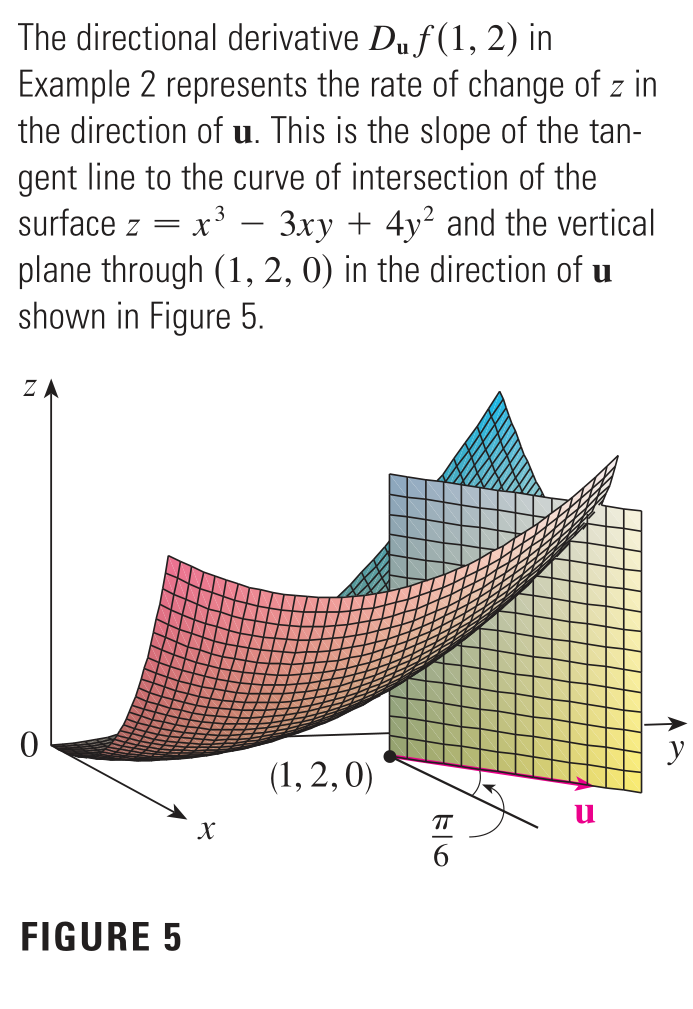
\includegraphics[width = 4.7 cm]{./images/grad2.png}
  
\end{minipage}
\begin{minipage}[]{0.67\linewidth}
{\fontfamily{lmtt}\selectfont \textbf{\textcolor{blue5}{\faIcon{map-marker-alt} EXAMPLE.}}} Find the directional derivative $D_uf(x,y)$ if \[f(x,y) = x^3 - 3xy + 4 y^2 \]
and \textbf{u} is given by $\theta = \pi/6$. What is $D_ \textbf{u} f(1,2)$?
 
{\fontfamily{lmtt}\selectfont \textbf{\textcolor{blue5}{SOLUTION.}}}  
$  f_x(x,y) = 3 x^2 - 3y \quad \text{ } \quad  f_y(x,y) = 8y -3 $

Therefore, 
\begin{equation*}
  \begin{split}
D_u f(x,y)  & = \cfrac{\sqrt{3 }}{2}(3 x^2 - 3y) + \cfrac{1 }{2 } (8y - 3)  \\
& = \cfrac{3 \sqrt{3 }}{2 } x^2 + \cfrac{4 - 3 \sqrt{3 }}{2 } y - \cfrac{3 }{ 2 }
  \end{split}
\end{equation*}
Hence $D_u f(1,2) = \cfrac{13 - 3 \sqrt{3 }}{2 }$
\end{minipage}
\pagebreak
\subsection*{{\fontfamily{lmss}\selectfont \textcolor{blue5}{\faIcon{anchor} \underline{The Gradient Vector}}}}
Notice that $D_ \textbf{u} = \langle f_x(x,y) , f_y(x,y) \rangle \cdot \textbf{u}$.
\begin{Def}[Gradient]
  The \textbf{gradient} of $f(x,y)$ is the vector function $\nabla f$ defined by 
  \[\nabla f(x,y) = \langle f_x (x,y) , f_y(x,y) \rangle = \cfrac{\partial f }{ \partial x } \textbf{i} + \cfrac{\partial f }{\partial y } \textbf{j}\]
  The directional derivative of $f(x,y)$ is $\quad D_ \textbf{u} f(x,y) = \nabla f(x,y) \cdot \textbf{u}$
\end{Def}
{\fontfamily{lmtt}\selectfont \textbf{\textcolor{blue5}{\faIcon{map-marker-alt} EXAMPLE.}}} If $f(x,y) = \sin{x} + e^{xy}$, then 
\begin{align*}
  & \nabla f(x,y) = \langle f_x, f_y  \rangle = \langle \cos{x} + y e^{xy}, xe^{xy} \rangle \\
  & \nabla f(0,1) = \langle 2, 0  \rangle
\end{align*}

\begin{minipage}[]{0.3\linewidth}
  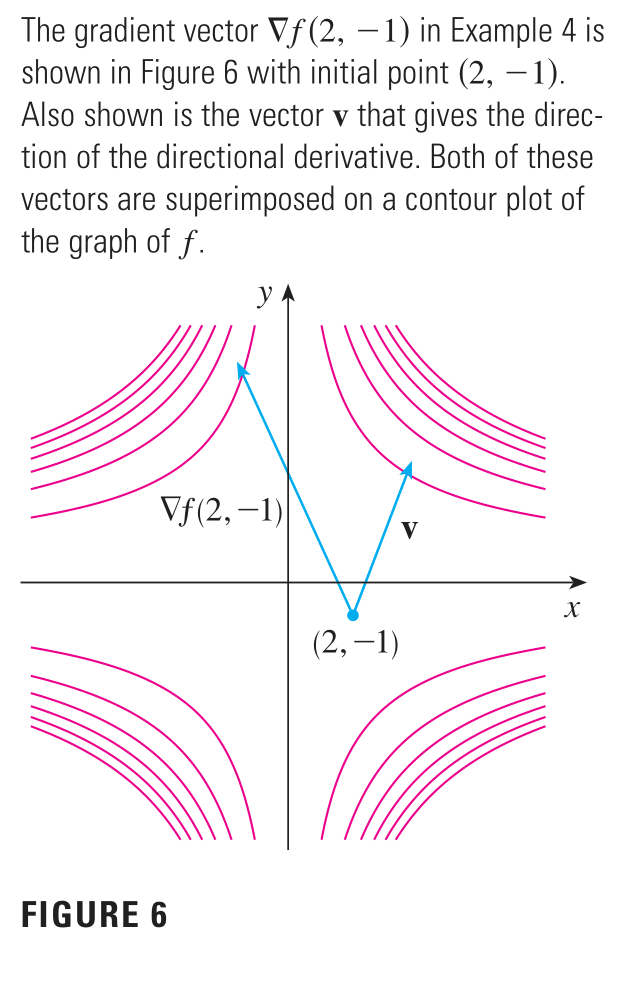
\includegraphics[width = 4.3 cm]{./images/grad4.png}
  
\end{minipage}
\begin{minipage}[]{0.67\linewidth}
  {\fontfamily{lmtt}\selectfont \textbf{\textcolor{blue5}{\faIcon{map-marker-alt} EXAMPLE.}}} Find the directional derivative of $f(x,y) = x^2 y^3 - 4y$ at $(2, -1 )$ in the direction of $\textbf{v} = 2 \textbf{i} + 5 \textbf{j}$.

  {\fontfamily{lmtt}\selectfont \textbf{\textcolor{blue5}{SOLUTION.}}} We first compute the gradient vector at $(2,-1)$: 
  \begin{align*}
    \nabla f(x,y) & = 2xy^3 \textbf{i} + (3 x^2 y^2 - 4 ) \textbf{i} \\
    \nabla f(2, -1) & = -4 \textbf{i} + 8 \textbf{j}
  \end{align*}
  The unit vector in the direction of \textbf{v} is $\textbf{u} = \cfrac{\textbf{v}}{|\textbf{v}|} = \cfrac{2 }{\sqrt{29 }} \textbf{ i} + \cfrac{5 }{\sqrt{29 }} \textbf{ j}$

  Therefore we have 
  \begin{align*}
    D_ \textbf{u} f(2,-1) & = \nabla f(2,-1) \cdot \textbf{u} = (-4 \textbf{i} + 8 \textbf{j}) \cdot \left( \cfrac{2 }{\sqrt{29 }} \textbf{ i} + \cfrac{5 }{\sqrt{29 }} \textbf{ j}  \right)\\
    & = \cfrac{-4 \cdot 2 + 8 \cdot 5  }{\sqrt{29}} = \cfrac{32 }{\sqrt{29 }}
  \end{align*}
\end{minipage}

\subsection*{{\fontfamily{lmss}\selectfont \textcolor{blue5}{\faIcon{anchor} \underline{Functions of Three Variables}}}}
\begin{Def}[Directional Derivatives]
  The \textbf{directional derivative} of $f$ at $(x_0, y_0, z_0)$ in the direction of a unit vector \textbf{u} $= \langle a, b, c  \rangle$ is 
  \[D_ \textbf{u} f(x_0, y_0, z_0) = \lim_{h \to 0 } \cfrac{f(x_0 + ha, y_0 + hb, z_0 + hc ) - f(x_0, y_0, z_0)}{h}\]
  The \textbf{gradient vector} is 
  \[\nabla f = \langle f_x, f_y, f_z  \rangle = \cfrac{\partial f }{ \partial x } \textbf{ i} + \cfrac{\partial f }{\partial y } \textbf{ j} + \cfrac{\partial f }{\partial z } \textbf{ k}  \]
  And the directional derivative is $\quad D_ \textbf{u} f(x,y,z) = \nabla f(x,y,z) \cdot \textbf{u}$
\end{Def} 
{\fontfamily{lmtt}\selectfont \textbf{\textcolor{blue5}{\faIcon{map-marker-alt} EXAMPLE.}}} If $f(x,y,z) = x \sin{yz}$, (a) find $\nabla f$ and (b) find $D_ \textbf{u} f(1,3,0)$ in the direction of $\textbf{v} = \textbf{i} + 2 \textbf{j}  - \textbf{k}$.

{\fontfamily{lmtt}\selectfont \textbf{\textcolor{blue5}{SOLUTION.}}} 
\[\nabla f = \sin{yz} \cdot \textbf{i} + xz\cos{yz} \cdot \textbf{j} + xy\cos{xz} \cdot \textbf{k}\]
The unit vector in the direction of \textbf{v} is 
\[\textbf{u} = \cfrac{1 }{\sqrt{6 }} \textbf{i} + \cfrac{2 }{\sqrt{6 }} \textbf{j} - \cfrac{1 }{\sqrt{6 }} \textbf{k}\]
Therefore 
\begin{align*}
  D _ \textbf{u} & = \nabla f(1,3,0) \cdot \textbf{u} \\
  & = 3 \textbf{k} \cdot \cfrac{1 }{\sqrt{6 }} \textbf{i} + \cfrac{2 }{\sqrt{6 }} \textbf{j} - \cfrac{1 }{\sqrt{6 }} \textbf{k} \\
  & = - \sqrt{\cfrac{3 }{2 }}
\end{align*}

\subsection{Maximizing the Directional Derivative}
\begin{Def}[Maximum Value of the Directional Derivative]
 The maximum value of $D_ \textbf{u} f(\textbf{x})$ is $|\nabla f(\textbf{x})|$, when \textbf{u} has the same direction as the gradient vector $\nabla f(\textbf{x})$.
\end{Def}

\begin{minipage}[]{0.3\linewidth}
  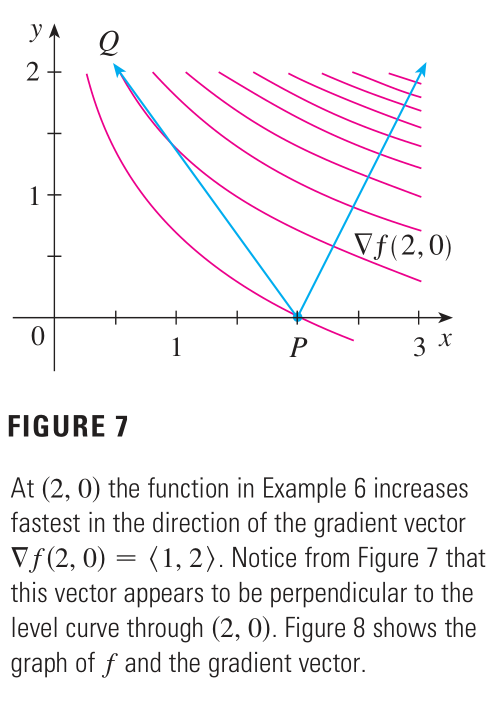
\includegraphics[width = 4.3 cm]{./images/maxeg6.png}
  
\end{minipage}
\begin{minipage}[]{0.67\linewidth}
  {\fontfamily{lmtt}\selectfont \textbf{\textcolor{blue5}{\faIcon{map-marker-alt} EXAMPLE.}}} 

  (a) If $f(x,y) = xe^y $, find the rate of change of $f$ at $P(2,0)$ in the direction from $P$ to $Q(\frac{1}{2}, 2 )$.

  (b) In what direction, $f$ has max $D _ \textbf{u} f$ and what's it?

  {\fontfamily{lmtt}\selectfont \textbf{\textcolor{blue5}{SOLUTION.}}} 

  (a) \begin{align*}
    \nabla f(x,y) & = \langle f_x, f_y  \rangle = \langle e^y, xe^y  \rangle \\
    \nabla f(2,0) & = \langle 1,2  \rangle
  \end{align*}
  The unit vector in the direction $\overrightarrow{PQ}$ is \textbf{u} $= \left< -\frac{3 }{5 }, \frac{4 }{5 }  \right>$, so we have 
  \begin{align*}
    D _ \textbf{u} f(2,0) & = \nabla f(2,0) \cdot \textbf{u} = \langle 1,2 \rangle \cdot  \left< -\frac{3 }{5 }, \frac{4 }{5 }  \right>  \\
    & = 1 \left( - \frac{3 }{5 } \right) + 2 \left( \frac{4 }{ 5 } \right) = 1
  \end{align*}

  (b) $f$ increases fastest in the direction of $\nabla f(2,0) = \langle 1, 2  \rangle$.
  \[|\nabla f(2,0)| = |\langle 1,2 \rangle  | = \sqrt{5 }\]
\end{minipage}

\subsection*{{\fontfamily{lmss}\selectfont \textcolor{blue5}{\faIcon{anchor} \underline{Tangent Planes to Level Surfaces}}}}

Suppose $S$ of $F(x,y,z) = k $, and $P(x_0, y_0, z_0) \in S$. We can write $\nabla F \cdot \textbf{r}'(t) = 0$ 
\[\nabla F (x_0, y_0, z_0) \cdot \textbf{r}'(t_0) = 0 \]
We see that the \textit{gradient vector} $\nabla F(x_0, y_0, z_0)$ is \textbf{perpendicular} to the tangent vector to any curve $C$ on $S$ that pass through $P$.

\begin{Def}[Tangent plane]
  If $\nabla F(x_0, y_0, z_0) \ne \textbf{0} $, there is a \textbf{tangent plane to the level surface $F(x,y,z) = k$ at $P(x_0, y_0, z_0)$} 
  \[F_x (x_0, y_0, z_0)(x - x_0) + F_y (x_0, y_0, z_0) ( y - y_0)  + F_z (x_0, y_0, z_0)(z - z_0)  = 0 \]
  The \textbf{normal line} to $S$ at $P$ is the line passing through $P$ and perpendicular to the tangent plane. The direction of it is given by $\nabla F(x_0, y_0, z_0)$ and its symmetric equation*s are 
  \[\cfrac{x - x_0 }{F_x (x_0, y_0, z_0)} = \cfrac{y - y_0 }{F_y (x_0, y_0, z_0)} = \cfrac{z - z_0 }{F_z (x_0, y_0, z_0)}\]
\end{Def}
{\fontfamily{lmtt}\selectfont \textbf{\textcolor{blue5}{{\small \faIcon{chevron-circle-right}} Special case.}}} When $z = f(x,y)$, then $F(x,y,z) = f(x,y) - z = 0$, we have 
\[f_x(x_0, y_0)(x - x_0) + f_y(x_0, y_0)(y - y_0) - (z - z_0) = 0\]
{\fontfamily{lmtt}\selectfont \textbf{\textcolor{blue5}{\faIcon{map-marker-alt} EXAMPLE.}}} Find the tangent plane and normal line at $(-2,1,-3)$ to the ellipsoid
\[\cfrac{x^2 }{4} + y^2 + \cfrac{z^2 }{9 } = 3 \]
{\fontfamily{lmtt}\selectfont \textbf{\textcolor{blue5}{SOLUTION.}}} The ellipsoid is the level surface ($k = 3 $) of the function 
\[F(x,y,z) = \cfrac{x^2 }{4 } + y^2 + \cfrac{z^2 }{9 }\]
Therefore we have 
\begin{align*}
  F_x(x,y,z) = \cfrac{x }{ 2 } & \quad & F_y(x,y,z) = 2y & \quad & F_z(x,y,z) = \cfrac{2z }{9 } \\
  F_x(-2, 1, -3 ) = -1 & \quad & F_y(-2, 1, -3)  = 2 & \quad & F_z(-2,1,-3) = - \cfrac{2 }{3 }
\end{align*}

\begin{minipage}[]{0.3\linewidth}
  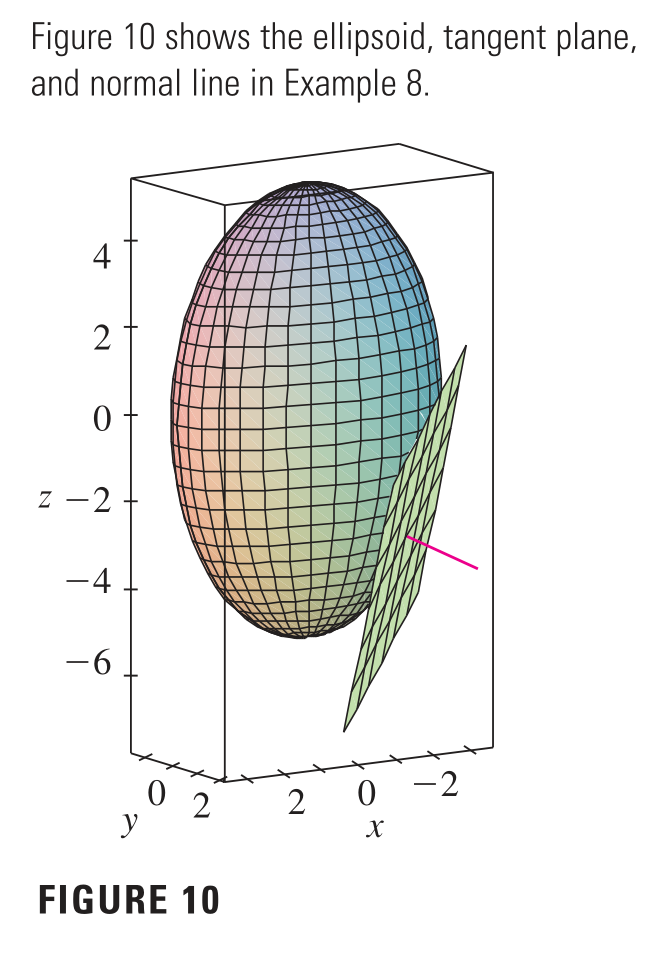
\includegraphics[width = 4.3 cm]{./images/fig10.png}
  
\end{minipage}
\begin{minipage}[]{0.67\linewidth}
The equation of the tangent plane at (-2, 1, -3) is 
\[-1(x + 2) + 2(y-1) - \cfrac{2}{3} (z + 3  ) = 0\]
The symmetric equations of the normal line are 
\[\cfrac{x + 2 }{ -1 } =  \cfrac{y - 1 }{2 } = \cfrac{z + 3 }{- \frac{2 }{3 }}\]
  
\end{minipage}

% \subsection*{{\fontfamily{lmss}\selectfont \textcolor{blue5}{\faIcon{anchor} \underline{Significance of the Gradient Vector}}}}
% Consider $f(x,y)$ and $P(x_0,y_0)$. Again $\nabla f(x_0, y_0)$ gives the direction of fastest increase of $f$. 

  \begin{minipage}[]{0.67\linewidth}
\subsection*{{\fontfamily{lmss}\selectfont \textcolor{blue5}{\faIcon{anchor} \underline{Maximum and Minimum Values}}}}
\begin{Def}[Local extrema]
\textbf{Local maximum} $f(a,b)$ if $f(x,y) \le f(a,b)$ when $(x,y)$ is near $(a,b)$.And the first-order partial derivatives of $f$ exists there, then $f_x(a,b) = 0$ and $f_y(a,b) = 0 $. 
\end{Def}
  
\end{minipage}
\begin{minipage}[]{0.3\linewidth}
  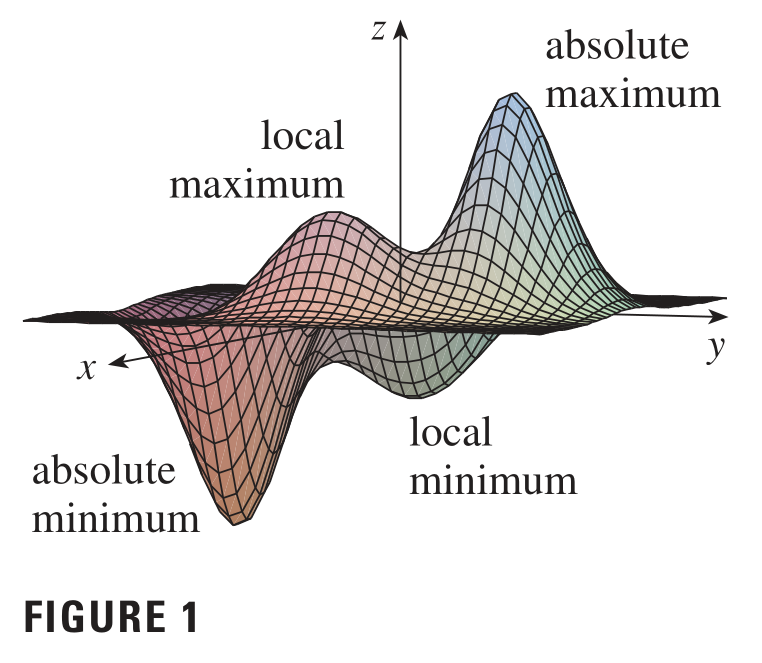
\includegraphics[width = 4.3 cm]{./images/localextrema.png}
  
\end{minipage}

If we put $f_x(a,b) = 0  $ and $f_y(a,b) = 0 $ in the equation of a tangent plane, we get $z = z_0$. So the tangent plane at a local extrema must be \textit{horizontal}.
A point $(a,b)$ is a \textbf{critical point} (or \textit{stationary point})  of $f$ if $f_x(a,b) = f_y(a,b) = 0$, or if one of these does not exist.

\begin{minipage}[]{0.3\linewidth}
  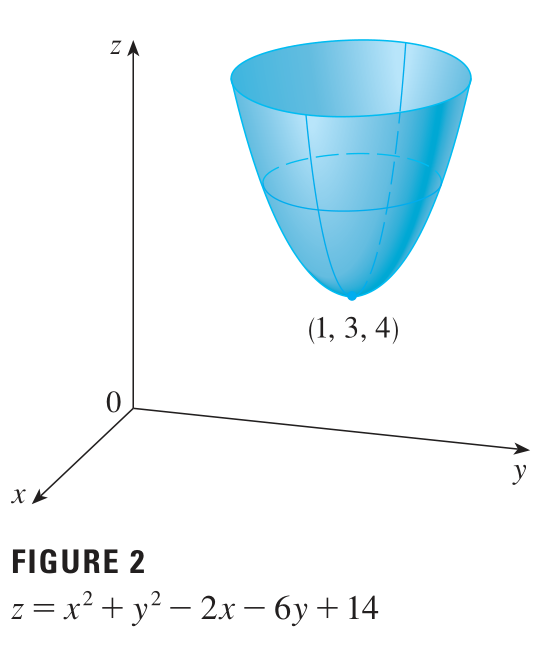
\includegraphics[width = 4.3 cm]{./images/min1}
  
\end{minipage}
\begin{minipage}[]{0.67\linewidth}

{\fontfamily{lmtt}\selectfont \textbf{\textcolor{blue5}{\faIcon{map-marker-alt} EXAMPLE.}}} Let $f(x,y) = x^2 + y^2 -2x - 6y + 14 $. Then 
\[f_x(x,y) = 2x - 2 \quad \text{ } \quad f_y(x,y) = 2y - 6 \]
These derivatives are equal to 0 when $x = 1, y = 3$. So the only critical point is $(1,3)$. 
\[f(x,y) = 4 + (x-1)^2 + (y-3)^2\]
We have $f(x,y) \ge 4 $. Therefore $f(1,3) = 4$ is a local minimum, and in fact it is the \textbf{absolute minimum} of $f$.
  
\end{minipage}

\begin{minipage}[]{0.3\linewidth}
  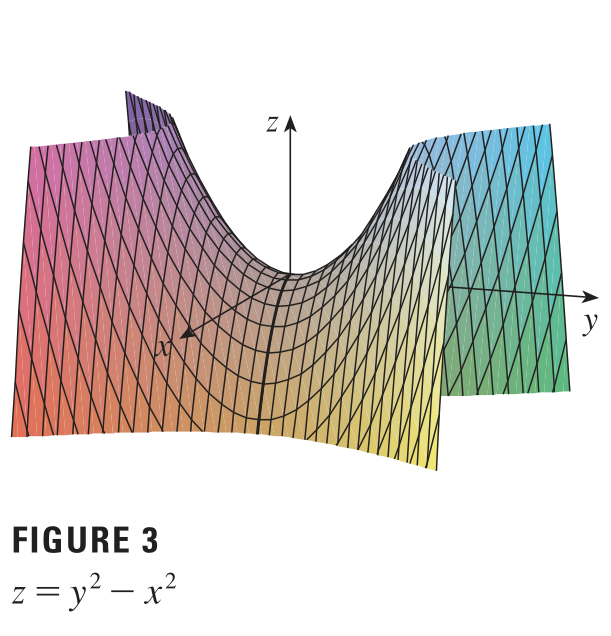
\includegraphics[width = 4.3 cm]{./images/saddle.png}
  
\end{minipage}
\begin{minipage}[]{0.67\linewidth}
  {\fontfamily{lmtt}\selectfont \textbf{\textcolor{blue5}{\faIcon{map-marker-alt} EXAMPLE.}}} Find the extreme values of $f(x,y) = x^2 + y^2 $.

 $f(x,y)$ is either maxima or minima depends on directions. So $(0,0)$ is a \textit{saddle point} of $f$. Then how to determine?
\end{minipage}

\begin{Def}[Second Derivatives Test]
  Suppose $f_x(a,b) = f_y(a,b) = 0 $. Let 
  \begin{align*}
  D & = D(a,b) = f_{xx}(a,b)f_{yy}(a,b) - [f_{xy}(a,b)]^2 \\
    & = \begin{vmatrix}
      f_{xx} & f_{xy} \\ 
      f_{yx} & f_{yy}
    \end{vmatrix} = f_{xx}f_{yy} - (f_{xy})^2
  \end{align*}
  (a) \textbf{Local minimum:} $D > 0, f_{xx}(a,b) > 0$.\\
  (b) \textbf{Local maximum:} $D > 0, f_{xx}(a,b) < 0$.\\
  (c) \textbf{Neither:} $D < 0$.
\end{Def}
{\fontfamily{lmtt}\selectfont \textbf{\textcolor{blue5}{\faIcon{greater-than} Note.}}} If $D = 0$, we have no idea.

\pagebreak

\begin{minipage}[]{0.3\linewidth}
  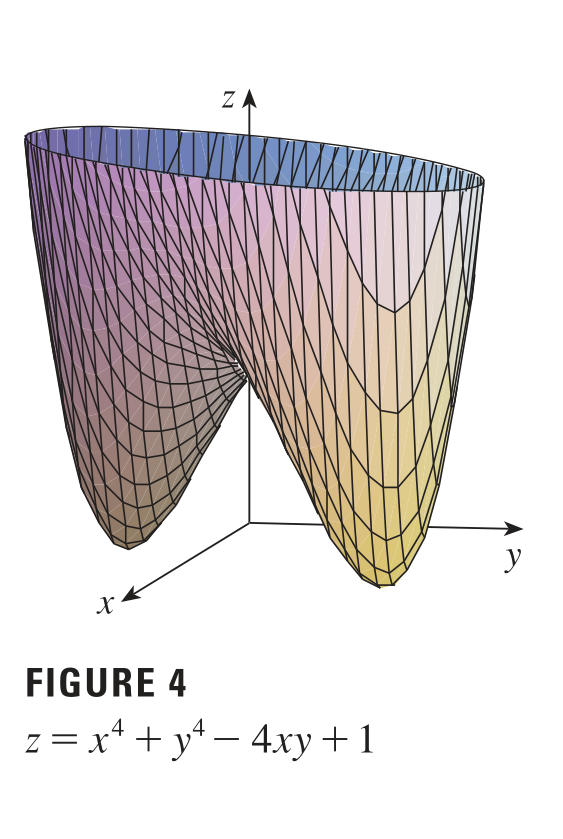
\includegraphics[width = 4.3 cm]{./images/min4.png}
  
\end{minipage}
\begin{minipage}[]{0.67\linewidth}
{\fontfamily{lmtt}\selectfont \textbf{\textcolor{blue5}{\faIcon{map-marker-alt} EXAMPLE.}}} Find the local maximum and minimum ad saddle points of $f(x,y) = x^4 + y^4 - 4xy + 1$.

First we have 
\begin{align*}
  f_x = 4x^3 - 4y & \quad & f_y = 4y^3 - 4x \\
  x^3 - y = 0 & \quad & y^3 - x = 0 
\end{align*}
which implies $0 = x^9 - x = x(x^2 - 1)(x^2 + 1)(x^4  + 1 )$, so there're 3 roots: 0, 1, -1. The 3 critical points are $(0,0), (1,1), (-1, -1)$.

Next we calculate the second partial derivatives and $D(x,y)$
\begin{align*}
  f_{xx} = 12x^2 & \quad & f_{xy} = -4 & \quad & f_yy = 12y^2 
\end{align*}
\[D(x,y) = f_{xx}f_{yy} - (f_{xy})^2 = 144 x^2 y^2 - 16 \]
Since $D(0,0) = -16 < 0$, it follows that (0,0) is a saddle point. And $D(1,1) = 128 >0, f_{xx}(1,1) = 12 > 0$, so it's a local minimum. Similarly, $(-1,-1)$ is a local minimum.
  
\end{minipage}\\
{\fontfamily{lmtt}\selectfont \textbf{\textcolor{blue5}{\faIcon{map-marker-alt} EXAMPLE.}}} Find the shortest distance from $(1,0,-2)$ to the plane $x + 2y + z = 4 $.

The distance from $(x,y,z )$ to $(1,0,-2 )$ is 
\[d^2 = f(x,y) = (x - 1)^2 + y^2 + (6-x-2y)^2   \]
By solving the equation 
\begin{align*}
  f_x = 4x + 4y -  14 = 0 \\
  f_y = 4x + 10y - 24 = 0 
\end{align*}
we find that the only critical point is $\left( \frac{11 }{6 }, \frac{5 }{3 } \right)$. Since $f_{xx} = 4, f_{xy} = 4, f_{yy} = 10 , D(x,y) = f_{xx}f_{yy} - (f_{xy})^2 = 24 > 0 $, so $f$ has a local minimum at $\left( \frac{11 }{6 }, \frac{5 }{3 } \right)$. There must be a point on the given plane that is closest to (1,0,-2). We also find that $d = \frac{5 }{6 } \sqrt{6 }$.


\subsection*{{\fontfamily{lmss}\selectfont \textcolor{blue5}{\faIcon{anchor} \underline{Absolute Maximum and Minimum Values}}}}
\begin{Def}[Extreme Value Theorem]
  If $f$ is continuous on a closed, bounded set $D \in \mathbb{R}^2$  then $f$ attains an absolute maximum value $f(x_1, y_1)$ and an absolute minimum value $f(x_2, y_2)$. 
  To find it, \\
  \textbf{\textcolor{blue5}{\fontfamily{lmss}\selectfont 1.}} Find the values of $f$ at the critical points of $f$ in $D$.\\
\textbf{\textcolor{blue5}{\fontfamily{lmss}\selectfont 2.}}  Find the extreme values of $f$ on the boundary of $D$.\\
\textbf{\textcolor{blue5}{\fontfamily{lmss}\selectfont 3.}}  Determine the largest and smallest ones.
\end{Def}

{\fontfamily{lmtt}\selectfont \textbf{\textcolor{blue5}{\faIcon{map-marker-alt} EXAMPLE.}}} Find the absolute maximum and minimum of $f(x,y) = x^2 - 2xy + 2y $ on the rectangle $D = \{(x,y) | \text{ }0 \le x \le 3, 0 \le y \le 2\}$.\\
Since $f$ is a polynominal, it's continuous on $D$. First find the critical points
\[f_x = 2x - 2y = 0 \quad \text{ } \quad f_y = -2x + 2 = 0 \]
So the only critical point is (1,1), and $f(1,1) = 1 $.

Now we look at the values of $f$ on the boundary of $D$, which consists of the four line segments $L_1, L_2, L_3, L_4$.

\begin{center}
  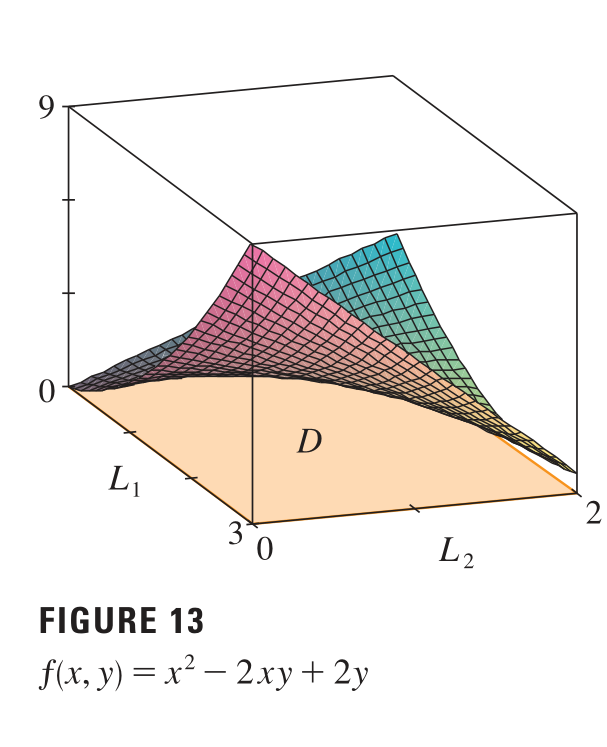
\includegraphics[width = 4.3 cm]{./images/fig13.png}
  
\end{center}

\begin{minipage}[]{0.3\linewidth}
  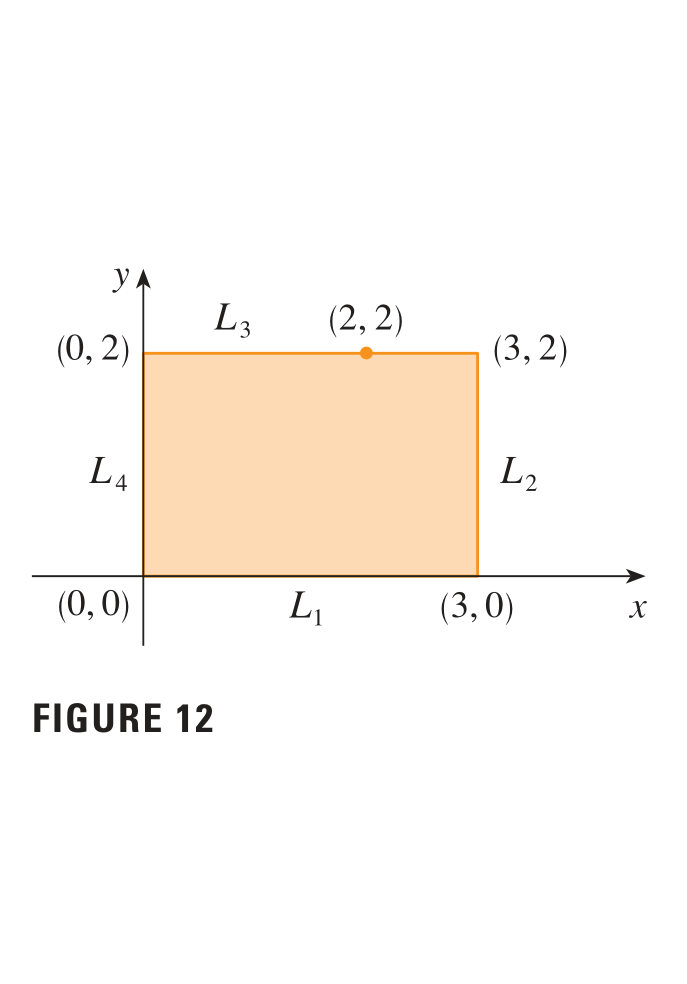
\includegraphics[width = 4.3 cm]{./images/rec12.png}
  
\end{minipage}
\begin{minipage}[]{0.67\linewidth}
 
\textcolor{blue5}{\small $\blacksquare$} On $L_1$, we have $y = 0 $ and 
\[f(x,0) = x^2 \quad \text{ } \quad 0 \le x \le 3 \]
Its minimum value is $f(0,0) = 0$ and maximum value is $f(3,0) = 9$.\\
\textcolor{blue5}{\small $\blacksquare$} On $L_2$, we have $x = 3$ and  
\[f(3, y) = 9  - 4y \quad \text{ } \quad 0 \le y \le 2   \]
The maximum value is $f(3,0) = 9 $ and the minimum value is $f(3,2) = 1$.\\
\textcolor{blue5}{\small $\blacksquare$} On $L_3$ we have $y = 2$ and 
\[f(x,2) = x^2 - 4x + 4 = (x- 2) ^2 \quad \text{ } \quad 0 \le x \le 3\]
The minimum value is $f(2,2) = 0$ and the maximum value is $f(0,2) = 4$.\\
\textcolor{blue5}{\small $\blacksquare$} On $L_4$ we have $x = 0$ and 
\[f(0,y) = 2y \quad \text{ } \quad 0 \le y \le 2 \]
with maximum value $f(0,2) = 4$ and minimum valye $f(0,0) = 0$.

Thus, on the boundary, the minimum value is 0 and the maximum is 9.

\end{minipage}

\begin{minipage}[]{0.3\linewidth}
  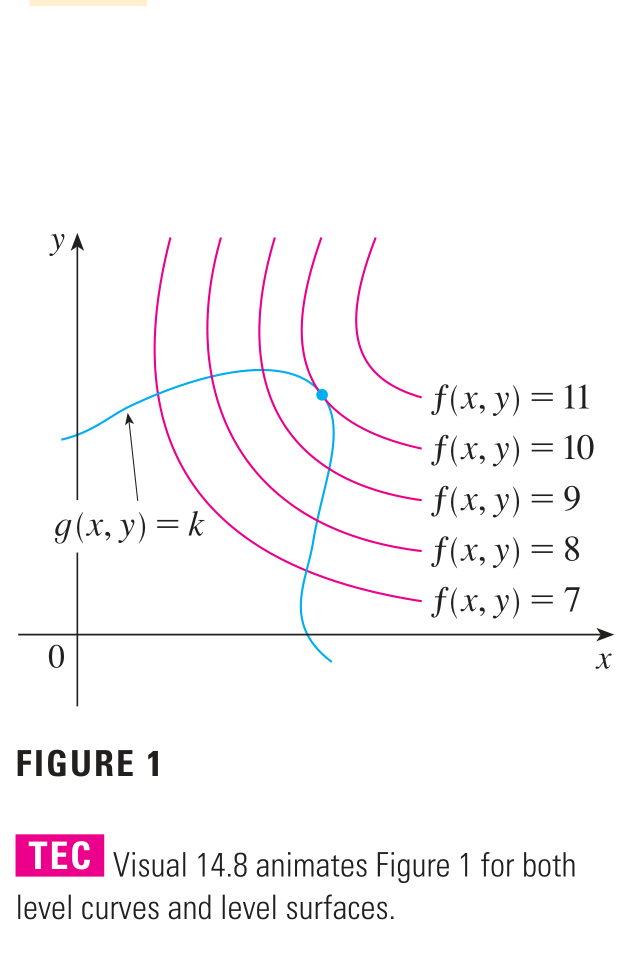
\includegraphics[width = 4.3 cm]{./images/lagrange.png}
  
\end{minipage}
\begin{minipage}[]{0.67\linewidth}
\subsection*{{\fontfamily{lmss}\selectfont \textcolor{blue5}{\faIcon{anchor} \underline{Lagrange Multipliers}}}}
We will discover Lagrange's methods for maximizing or minimizing a general function $f(x,y,z)$ to a constraint (or side contidition) of the form $g(x,y,z) = k$.
\end{minipage}

\begin{Def}[Method of Lagrange Multipliers]
  To find the maximum and minimum values of $f(x,y,z)$ to the constraint $g(x,y,z) = k$ (assume they exist and $\nabla g \ne \textbf{0}$ on the surface $g(x,y,z) = k$):\\
  (a) Find all $x,y,z$ and $\lambda $ (\textbf{Lagrange multiplier}) such that 
  \begin{align*}
    \nabla f(x,y,z) & = \lambda \nabla g(x,y,z) \\
    g(x,y,z) & = k 
  \end{align*}
  (b) Evaluate $f$ at all these points and find the largest and smallest ones.
\end{Def}  
Write (a) in terms of components 
\[f_x = \lambda g_x \quad \text{ } \quad f_y = \lambda g_y \quad \text{ } \quad f_z = \lambda g_z \quad \text{ } \quad g(x,y,z) = k\]
It's not necessary to find explicit values for $\lambda $.\\
{\fontfamily{lmtt}\selectfont \textbf{\textcolor{blue5}{\faIcon{map-marker-alt} EXAMPLE.}}} A rectangular box without a lid is to be made from 12 m$^2$ of cardboard. Find the maximum volume.

{\fontfamily{lmtt}\selectfont \textbf{\textcolor{blue5}{SOLUTION.}}}  We wish to maximize $V = xyz$, where $x,y,z$ are the length, width and height of the box, subject to the constraint 
\[g(x,y,z) = 2xz + 2yz + xy = 12\]
We look for $x,y,z, \lambda $ that $\nabla V = \lambda \nabla g$ and $g(x,y,z) = 12$. 
\begin{align*}
  V_x = \lambda g_x \\
  V_y = \lambda g_y \\ 
  V_z = \lambda g_z \\
  2xz + 2yz + xy = 12 
\end{align*}
which become 
\begin{align*}
  yz = \lambda (2z + y) \\
  xz = \lambda (2z + x) \\
  xy = \lambda (2x + 2y) \\
  2xz + 2yz + xy = 12 
\end{align*}
Observe that $\lambda \ne 0$, and we have $2xz + xy = 2yz + xy$ which gives $xz = yz$. But $z \ne 0 $, or $V = 0 $. So $x = y$. We also have $x = y = 2z$.
\[4 z^2 + 4 z^2 + 4 z^2 = 12 \]
Therefore we have $x = y =2$, and $z = 1$.

\begin{minipage}[]{0.3\linewidth}
  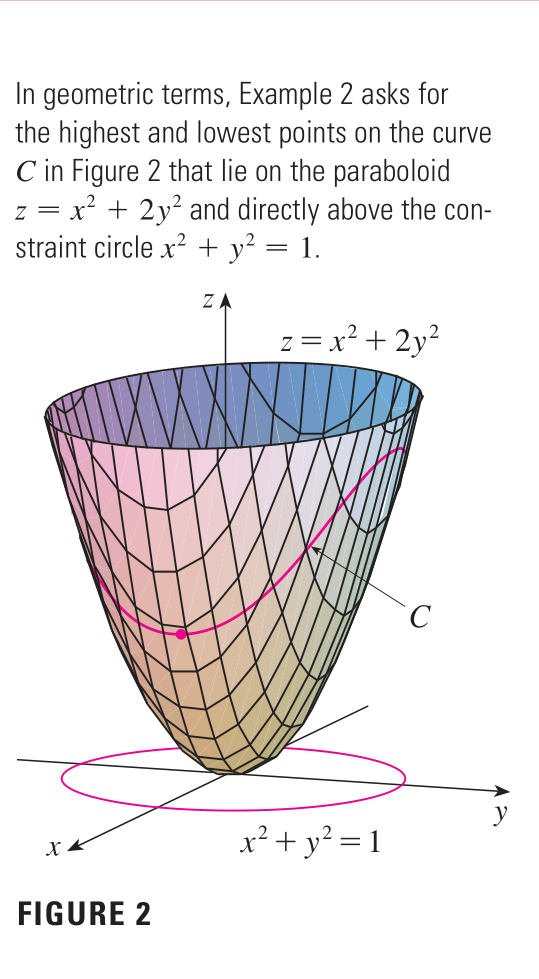
\includegraphics[width = 4.3 cm]{./images/lagrange2.png}\\
  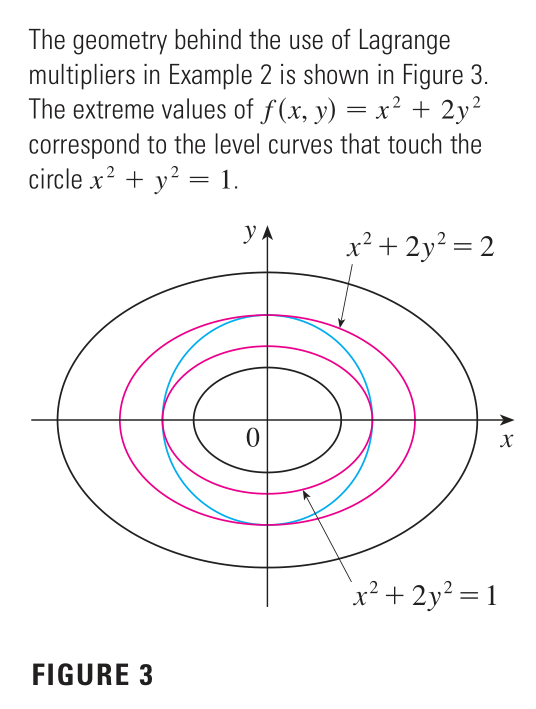
\includegraphics[width = 4.3 cm]{./images/lagrange3.png}
  
  
\end{minipage}
\begin{minipage}[]{0.67\linewidth}
  {\fontfamily{lmtt}\selectfont \textbf{\textcolor{blue5}{\faIcon{map-marker-alt} EXAMPLE.}}} Find the extreme values of $f(x,y) = x^2 + 2 y^2 $ on the circle $x^2 + y^2 = 1 $.  

  Solve the equation 
  \begin{align*}
  f_x = \lambda g_x, \quad & f_y = \lambda g_y, \quad g(x,y) = 1\\
   &  2x = 2x \lambda \\
   &  4y = 2y \lambda \\
   &  x^2 + y^2 = 1 
  \end{align*}
\textcolor{blue5}{\small $\blacksquare$} $x = 0$, then $y = \pm 1$.\\
\textcolor{blue5}{\small $\blacksquare$} $\lambda = 1$, then $y = 0$, and $x = \pm 1$.\\
Evaluating $f$ at these 4 points, we find that $f_ \text{max} = f(0, \pm 1) = 2$ and $f_ \text{min} = f(\pm 1, 0) = 1 $.
\end{minipage}

{\fontfamily{lmtt}\selectfont \textbf{\textcolor{blue5}{\faIcon{map-marker-alt} EXAMPLE.}}} Find the points on the sphere $x^2 + y^2 + z^2 = 4 $ that are closest and farthest from $(3,1,-1)$.
\end{document}

